\documentclass[UTF8]{ctexbook}
\usepackage[a4paper, left = 3cm, right = 3cm, top = 3cm, bottom = 3cm]{geometry}
\usepackage{amsmath} %数学公式
\usepackage{amssymb}             %数学公式
\usepackage{amsfonts}            %数学字体
\usepackage{mathrsfs}            %数学花体
\usepackage{graphicx}

\title{频率域滤波的数学基础}
\author{玩味者}
\begin{document}
	\maketitle
	\tableofcontents
	\chapter{傅里叶变换的理论部分}
		\section{傅里叶级数的复数形式}
			在微积分课程中已经知道,一个周期函数如果满足Dirichlet条件,便可以表达为如下的三角无穷级数形式:
			\begin{equation}
				\begin{split}
					&f(t)=\dfrac{a_0}{2}+\sum_{n = 1}^\infty(a_n\cos n\omega t+b_n\sin n\omega t)\quad t\in [-\dfrac{T}{2}, \dfrac{T}{2}]\\
					&\omega= \dfrac{2\pi}{T},\\
					&a_0=\dfrac{2}{T}\int_{-\frac{T}{2}}^{\frac{T}{2}}f(t)\ dt,\\
					&a_n=\dfrac{2}{T}\int_{-\frac{T}{2}}^{\frac{T}{2}}f(t)\cos n\omega t\ dt,\\
					&b_n=\dfrac{2}{T}\int_{-\frac{T}{2}}^{\frac{T}{2}}f(t)\sin n\omega t\ dt,\\
				\end{split}
			\end{equation}

			以上的形式称为函数的傅里叶级数展开式(三角形式)。

			一个函数被分解为两种三角函数的无穷和,这种形式的使用是不方便的,如果能变成同一个函数的无穷和,事情就会简单很多。于是引入欧拉公式:
			\begin{equation}
				e^{i\theta}=\cos \theta +i \sin\theta
			\end{equation}

			由(1.2)式可以很容易推导出
			\begin{equation}
				\cos\theta =\dfrac{e^{i\theta}+e^{-i\theta}}{2}\quad \sin\theta = \dfrac{e^{i\theta}-e^{-i\theta}}{2i}
			\end{equation}

			将(1.3)代入(1.1)
			\begin{equation}
				\begin{split}
					f(t)&=\dfrac{a_0}{2}+\sum\limits_{n = 1}^\infty(a_n\dfrac{e^{in\omega t}+e^{-in\omega t}}{2}+b_n\dfrac{e^{in\omega t}-e^{-in\omega t}}{2i})\\
					&= \dfrac{a_0}{2}+\sum\limits_{n = 1}^\infty(\dfrac{a_n-i b_n}{2}e^{in\omega t}+\dfrac{a_n+i b_n}{2}e^{-in\omega t})
				\end{split}
			\end{equation}
			
			根据傅里叶系数的三角形式和(1.2)的比较,可以知道
			\begin{equation}
				\begin{split}
					&\begin{split}
						a_n+ib_n&=\dfrac{2}{T}\int_{-\frac{T}{2}}^{\frac{T}{2}}f(t)\cos n\omega t\ dt+i\dfrac{2}{T}\int_{-\frac{T}{2}}^{\frac{T}{2}}f(t)\sin n\omega t\ dt\\
						&= \dfrac{2}{T}\int_{-\frac{T}{2}}^{\frac{T}{2}}f(t)(\cos n\omega t+i\sin n\omega t)\ dt\\
						&= \dfrac{2}{T}\int_{-\frac{T}{2}}^{\frac{T}{2}}f(t)e^{in\omega t}\ dt
					\end{split}\\
					&a_n-ib_n=\dfrac{2}{T}\int_{-\frac{T}{2}}^{\frac{T}{2}}f(t)e^{-in\omega t}\ dt
				\end{split}
			\end{equation}

			$n=0$时,(1.5)式将退化为(1.1)式中$a_0$的形式,令
			\begin{equation}
				c_n=\dfrac{1}{T}\int_{-\frac{T}{2}}^{\frac{T}{2}}f(t)e^{-in\omega t}\ dt, \quad \omega_n=n\omega
			\end{equation}

			这样就可以把三角形式的系数全部转成
			\begin{equation}
				\dfrac{a_0}{2}=c_0,\quad
				\dfrac{a_n+ib_n}{2}=c_{-n},\quad
				\dfrac{a_n-ib_n}{2}=c_{n}
			\end{equation}

			所以
			\begin{equation}
				\begin{split}
					f(t)&= c_0+\sum\limits_{n=1}^\infty[c_n e^{i\omega_n t}+c_{-n}e^{i\omega_{-n} t}]\\
					&= \sum\limits_{n=-\infty}^{\infty}c_n e^{i\omega_n t}
				\end{split}
			\end{equation}

			于是,结合(1.8)和(1.6),我们得到了\textbf{傅里叶级数的复数形式}\footnote{其实,非周期函数可以看作是周期为$[-\infty, \infty]$的周期函数,此时,任意函数(这里并不严格)都可以满足(1.8)式}

		\section{傅里叶积分公式}
			当周期$T$无穷大的时候,有
			\begin{equation}
				\lim_{T\to +\infty}f_T(t)=f(t)
			\end{equation}

			那么,根据(1.8)式,一个非周期函数$f(t)$就有
			\begin{equation}
				f(t)=\lim_{T\to +\infty}\sum\limits_{n=-\infty}^{\infty}\left[\dfrac{1}{T}\int_{-\frac{T}{2}}^{\frac{T}{2}}f(\tau)e^{-i\omega_n \tau}\ d\tau\right] e^{i\omega_n t}
			\end{equation}

			当$n$取一切整数的时候,$\omega_n$所对应的点便均匀地分布在整个数轴上
			\begin{equation}
				\Delta\omega_n=\omega_n-\omega_{n - 1}=\dfrac{2\pi}{T}\Rightarrow T=\dfrac{2\pi}{\Delta\omega_n}
			\end{equation}
			
			当$T\to +\infty$时,$\Delta\omega_n\to 0$,所以(1.10)可以写作
			\begin{equation}
				f(t)=\lim_{\Delta\omega_n\to 0}\sum\limits_{n=-\infty}^{\infty}\left[\dfrac{1}{2\pi}\left(\int_{-\infty}^{\infty}f(\tau)e^{-i\omega_n \tau}\ d\tau\right)e^{i\omega_n t}\right] \Delta\omega_n
			\end{equation}
			
			把式子排列成上面这种形式是有原因的,把中括号内部的部分看作是一个关于$\omega_n$的函数,那么整个式子正好是定积分的定义式,于是(12)式可以写成下面的形式
			\begin{equation}
				f(t)=\dfrac{1}{2\pi}\int_{-\infty}^{\infty}\left[\int_{-\infty}^{\infty}f(\tau)e^{-i\omega \tau}\ d\tau\right] e^{i\omega t} d\omega
			\end{equation}
			
			将(1.13)式称为\textbf{傅里叶积分公式}

		\section{傅里叶变换}

			由(1.13)式可以直接得出傅里叶变换的形式,设中括号内部的部分为
			\begin{equation}
				F(\omega)=\int_{-\infty}^{\infty}f(t)e^{-i\omega t}\ dt
			\end{equation}

			那么,把(1.14)代入(1.13)
			\begin{equation}
				f(t)=\dfrac{1}{2\pi}\int_{-\infty}^{\infty}F(\omega) e^{i\omega t} d\omega
			\end{equation}

			这里,(1.14)被称为$f(t)$的\textbf{傅里叶变换式}\footnote{当然,在工程中也有使用如下形式的傅里叶变换
				$$
				F(\omega)=\sqrt{\dfrac{1}{2\pi}}\int_{-\infty}^{\infty}f(t)e^{-i\omega t}\ dt\\
				f(t)=\sqrt{\dfrac{1}{2\pi}}\int_{-\infty}^{\infty}F(\omega) e^{i\omega t} d\omega
				$$
				这样可以使得系数均衡(强迫症福利),这个都是人为定义的,系数的改变并不影响其数学性质},记作
			\begin{equation}
				F(\omega)=\mathscr{F}[f(t)]
			\end{equation}

			反之,(1.15)被称为$F(\omega)$的\textbf{傅里叶逆变换式},记作
			\begin{equation}
				f(t)=\mathscr{F}^{-1}[F(\omega)]
			\end{equation}
			
			在信号处理的时候,一个连续的信号可以看作是$f(t)$,这是以时间为自变量的函数,而它的傅里叶变换$F(\omega)$是以$\omega$为自变量的函数,或者说,是频率的函数($\omega=2\pi f$)

		\section{傅里叶变换的性质}

			傅里叶变换的形式是很美好的,简单明了。但是要应用这个结论,需要找到它的一些性质。以下讨论都假设$f(t)$是符合傅里叶变换要求的函数

			\begin{enumerate}
				\item{线性性质}
					由于积分的线性性质,傅里叶变换很自然也具有线性性质
					\begin{equation}
						\begin{split}
							&\mathscr{F}[\alpha f_1(t)+\beta f_2(t)] = \alpha F_1(\omega)+\beta F_2(\omega)\\
							&\mathscr{F}^{-1}[\alpha F_1(\omega)+\beta F_2(\omega)] = \alpha f_1(t)+\beta f_2(t)
						\end{split}
					\end{equation}

				\item{位移性质}
					\begin{equation}
						\begin{split}
							&\begin{split}
								\mathscr{F}[f(t\pm t_0)]&=\int_{-\infty}^{\infty}f(t\pm t_0)e^{-i\omega t}\ dt\\
								&= \int_{-\infty}^{\infty}f(u)e^{-i\omega (u\mp t_0)}\ du\\
								&= e^{\pm i\omega t_0}\int_{-\infty}^{\infty}f(u)e^{-i\omega u}\ du\\
								&= e^{\pm i\omega t_0}F(\omega)
							\end{split}\\
							&\mathscr{F}^{-1}[F(\omega\mp\omega_0)]=e^{\pm i\omega_0 t}f(t)
						\end{split}
					\end{equation}
					上面的这个结论说明,函数在时域或频域上的位移相当于相对的域中的函数乘以一个因子(加减$\to$乘除)

				\item{微分性质}
					\begin{equation}
						\begin{split}
							\mathscr{F}[f'(t)]&=\int_{-\infty}^{\infty}f'(t)e^{-i\omega t}\ dt\\
							&=\int_{-\infty}^{\infty}e^{-i\omega t}\ df(t)\\
							&=f(t)e^{-i\omega t}|_{-\infty}^{\infty}-\int_{-\infty}^{\infty}f(t)\ de^{-i\omega t}\\
							&=f(t)e^{-i\omega t}|_{-\infty}^{\infty}+i\omega\int_{-\infty}^{\infty}f(t)e^{-i\omega t}\ dt\\
						\end{split}
					\end{equation}
					做到这一步做不下去了,因为如果不给$f(t)$再加上额外的限制的话,$f(t)e^{-i\omega t}|_{-\infty}^{\infty}$这一项就会变成无穷大,所以,必须给$f(t)$加一个限制
		
					\begin{quote}
						$f(t)$在$(-\infty, \infty)$上连续或只有有限个可去间断点,且当$|t|\to +\infty$时,$f(t)\to 0$
					\end{quote}
		
					有了这个限制之后,前面那一项等于0,得到
					\begin{equation}
						\begin{split}
						\mathscr{F}[f'(t)]&=i\omega\int_{-\infty}^{\infty}f(t)e^{-i\omega t}\ dt\\
						&=i\omega\mathscr{F}[f(t)]
						\end{split}
					\end{equation}
		
					用类似的方法(限制条件),可以得到
					\begin{equation}
						\mathscr{F}^{-1}[F'(\omega)]=-it\mathscr{F}^{-1}[F(\omega)]
					\end{equation}
					这个性质是很有用的,它把一个函数的求导变成了对应域中的乘因子
		
					使用数学归纳法可以很容易证明,对于$n$阶微分也有该性质,区别在于对因子求$n$次幂
		
					在求导方便的时候,可以用这种方法来求$t^nf(t)$形式函数的傅里叶变换结果;反之,则可以用傅里叶变换求出导数

				\item{积分性质}
					\begin{equation}
						\begin{split}
							\begin{split}
							\mathscr{F}[f(t)]&=\mathscr{F}[\dfrac{d}{dt}\int_{-\infty}^tf(t)\ dt]\\
							&= i\omega\mathscr{F}[\int_{-\infty}^tf(t)\ dt]
							\end{split}\\
							\Rightarrow\mathscr{F}[\int_{-\infty}^tf(t)\ dt]=\dfrac{1}{i\omega}\mathscr{F}[f(t)]
						\end{split}
					\end{equation}
					同理
					\begin{equation}
						\mathscr{F}^{-1}[\int_{-\infty}^\omega F(\omega)\ d\omega]=-\dfrac{1}{it}\mathscr{F}^{-1}[F(\omega)]
					\end{equation}
					和微分性质类似,这里不再赘述

				\item{乘积定理}
					设$F_1(\omega) = \mathscr{F}[f_1(t)]$,$F_2(\omega) = \mathscr{F}[f_2(t)]$,则
					\begin{equation}
						\begin{split}
							&\int_{-\infty}^{\infty}\overline{f_1(t)}f_2(t)dt=\dfrac{1}{2\pi}\int_{-\infty}^{\infty}\overline{F_1(\omega)}F_2(\omega)d\omega\\
							&\int_{-\infty}^{\infty}f_1(t)\overline{f_2(t)}dt=\dfrac{1}{2\pi}\int_{-\infty}^{\infty}F_1(\omega)\overline{F_2(\omega)}d\omega
						\end{split}
					\end{equation}
					这个结论很有意思,这说明原函数的乘积之积分和变换之后的乘积之积分仅有一个系数的差异(如果按照另外一种傅里叶变换的定义,则这个系数差异也没有)

				\item{能量积分}
					如果在上一个性质中,两个函数一样,那么可以得到
					\begin{equation}
						\int_{-\infty}^{\infty}[f(t)]^2\ dt=\dfrac{1}{2\pi}\int_{-\infty}^{\infty}|F(\omega)|^2\ d\omega
					\end{equation}
					这个结论是非常重要的,称为Parseval等式,令
					\begin{equation}
						S(\omega)=|F(\omega)|^2
					\end{equation}
					称为\textbf{能量密度函数}或\textbf{能量谱密度},由它可以决定函数$f(t)$的能量分布规律
		
					这里说$[f(t)]^2$是能量密度,或者说信号的“功率”,这是需要解释的:
					
					所谓功率,在物理上的定义是单位时间内做功的多少,以如下式定义:
					\begin{equation}
					P = \dfrac{W}{t}
					\end{equation}
					更进一步,我们假设这个函数是一个电信号的抽象。在电路中:
					\begin{equation}
					P = UI = I^2R = \dfrac{U^2}{R}
					\end{equation}
					以上面的式子来看,信号幅值的度量是用电压的高低表示的,如果把电路中的电阻值视为单位1,那么输出信号的瞬时功率就是
					\begin{equation}
					P = U^2
					\end{equation}
					一段时间内的功率就应该对其在时间上积分,所以,用信号的平方表示信号的功率是恰当的
			\end{enumerate}

		\section{卷积定理}
			卷积的定义是:
			\begin{equation}
				f_1(t)*f_2(t) = \int_{-\infty}^{+\infty}f_1(\tau)f_2(t - \tau)\ d\tau
			\end{equation}
			下面结合(14),我们对两个函数的卷积进行傅里叶变换:
			\begin{equation}
				\begin{split}
				\mathscr{F}[f_1(t)*f_2(t)] &= \mathscr{F}[\int_{-\infty}^{+\infty}f_1(\tau)f_2(t - \tau)\ d\tau]\\
				&= \int_{-\infty}^{+\infty}\int_{-\infty}^{+\infty}f_1(\tau)f_2(t - \tau)\ d\tau\ e^{-i\omega t}\ dt\\
				&= \int_{-\infty}^{+\infty}\int_{-\infty}^{+\infty}f_1(\tau)f_2(t - \tau)e^{-i\omega (\tau + t -\tau)}\ d\tau dt\\
				&= \int_{-\infty}^{+\infty}\int_{-\infty}^{+\infty}f_1(\tau)e^{-i\omega \tau}f_2(t - \tau)e^{-i\omega (t - \tau)}\ d\tau dt\\
				&= \int_{-\infty}^{+\infty}\int_{-\infty}^{+\infty}f_1(\tau)e^{-i\omega \tau}f_2(t - \tau)e^{-i\omega (t - \tau)}\ dt d\tau\\
				&= \int_{-\infty}^{+\infty}f_1(\tau)e^{-i\omega \tau}d\tau\int_{-\infty}^{+\infty}f_2(t - \tau)e^{-i\omega (t - \tau)}\ dt\\
				&= \mathscr{F}[f_1(t)]\cdot\mathscr{F}[f_2(t)]
				\end{split}
			\end{equation}
			同理可得
			\begin{equation}
				\begin{split}
					\mathscr{F}[f_1(t)\cdot f_2(t)] &= \dfrac{1}{2\pi}\int_{-\infty}^{\infty}F_1(\omega) e^{i\omega t} d\omega\ \dfrac{1}{2\pi}\int_{-\infty}^{\infty}F_2(\omega) e^{i\omega t} d\omega\\
					&= \dfrac{1}{(2\pi)^2}\int_{-\infty}^{\infty}F_1(\tau) e^{i\tau t} d\tau\ \int_{-\infty}^{\infty}F_2(\omega - \tau) e^{i(\omega - \tau) t} d(\omega - \tau)\\
					&= \dfrac{1}{(2\pi)^2}\int_{-\infty}^{\infty}\int_{-\infty}^{\infty}F_1(\tau) e^{i\tau t} F_2(\omega - \tau) e^{i(\omega - \tau) t}\ d\tau d\omega\\
					&= \dfrac{1}{(2\pi)^2}\int_{-\infty}^{\infty}\left[\int_{-\infty}^{\infty}F_1(\tau) F_2(\omega - \tau)\ d\tau\right]e^{i\omega t}d\omega\\
					&= \dfrac{1}{(2\pi)^2}\int_{-\infty}^{\infty}\left[F_1(\omega)*F_2(\omega)\right]e^{i\omega t}d\omega\\
					&= \dfrac{1}{2\pi}\mathscr[F_1(\omega)*F_2(\omega)]
				\end{split}
			\end{equation}
			我们称(33)式为\textbf{时域的卷积定理},称(34)式为\textbf{频域的卷积定理}

	\chapter{一些特殊函数的傅里叶变换}
		\section{方波}
			\begin{equation}
				f(t)=E, \quad t\in \left[-\frac{\tau}{2}, \frac{\tau}{2}\right]
			\end{equation}
			下面求$f(t)$的傅里叶变换结果
			\begin{equation}
				\begin{split}
					\mathscr{F}[f(t)] &= \int_{-\infty}^{\infty}f(t)e^{-i\omega t}\ dt\\
					&= \int_{-\infty}^{\infty}E\ e^{-i\omega t}\ dt\\
					&= -\dfrac{E}{i\omega}e^{-i\omega t}|_{-\frac{\tau}{2}}^{\frac{\tau}{2}}\\
					&= \dfrac{E}{i\omega}(e^{i\omega \frac{\tau}{2}}-e^{-i\omega\frac{\tau}{2}})\\
				\end{split}
			\end{equation}
			上式利用欧拉定理(2),得到
			\begin{equation}
				\begin{split}
					\mathscr{F}[f(t)] &= \dfrac{E}{i\omega}(e^{i\omega \frac{\tau}{2}}-e^{-i\omega\frac{\tau}{2}})\\
					&= \dfrac{E}{i\omega}(\cos (\omega \dfrac{\tau}{2}) +i \sin(\omega \dfrac{\tau}{2})-\cos (-\omega \dfrac{\tau}{2}) -i \sin(-\omega \dfrac{\tau}{2}))\\
					&= \dfrac{E}{i\omega}(i \sin(\omega \dfrac{\tau}{2}) +i \sin(\omega \dfrac{\tau}{2}))\\
					&= \dfrac{2E}{\omega}\sin\dfrac{\omega\tau}{2}\\
				\end{split}
			\end{equation}
			图\ref{fig1}是由Mathematica生成的图像,表示$E = 1, \tau = 1$时的图像
			
			\begin{figure}[h]
				\centering
				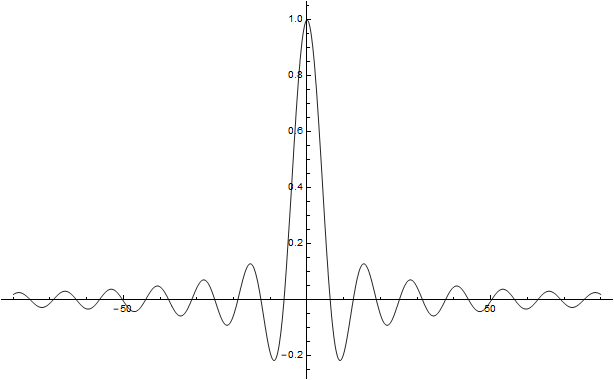
\includegraphics[scale=0.3]{1.png}
				\caption{方波的傅里叶变换}
				\label{fig1}
			\end{figure}

			应当注意到,这个函数是$\dfrac{\sin x}{x}$的变形,在$x=0$的时候是没有定义的

		\section{$\delta$-函数}

			这是一种广义的函数由一个描述和一个积分式共同定义
			\begin{equation}
				\delta(t) = \left\{
				\begin{aligned}
				\infty & \qquad t=0\\
				0& \qquad else 
				\end{aligned}
				\right.
			\end{equation}
			并且
			\begin{equation}
				\int_{-\infty}^{\infty}\delta(t)\ dt=\int_{0}^{\epsilon}\dfrac{1}{\epsilon}\ dt=1
			\end{equation}

			这个函数没办法用图像表示出来,因为它在$t = 0$的时候有一个无穷大的冲激,而在其他地方值为0,就好像用钉子钉墙,一个能量恒定的冲激作用在一个面积很小的点上,而其他的地方则没有能量作用。故这个函数又叫做冲激函数。

			下面证明,$\delta$-函数具有采样性质:
			\begin{equation}
				\int_{-\infty}^{\infty}\delta(t-t_0)f(t)\ dt=f(t_0)
			\end{equation}

			设$f(t)$是一个在$t_0$处连续的函数
			\begin{equation}
				\int_{-\infty}^{\infty}\delta(t-t_0)f(t)\ dt = \lim_{\epsilon\to 0}\dfrac{1}{\epsilon}\int_{t_0}^{t_0+\epsilon}f(t)\ dt
			\end{equation}
			
			利用积分中值定理
			\begin{equation}
				\int_{a}^{b}f(x)\ dx = f(\epsilon) (b - a)\qquad a\leq\epsilon\leq b
			\end{equation}
			可以得到
			\begin{equation}
				\int_{-\infty}^{\infty}\delta(t-t_0)f(t)\ dt = f(\tau)\qquad \tau\in\left[t_0, t_0 + \epsilon\right]
			\end{equation}
			由于$\epsilon\to 0$,所以
			\begin{equation}
				\int_{-\infty}^{\infty}\delta(t-t_0)f(t)\ dt = f(t_0)
			\end{equation}
			
			命题得证

			证明了这个性质之后,它的傅里叶变换便可以直接得出来:
			\begin{equation}
				\mathscr{F}[\delta(t)]=\int_{-\infty}^{\infty}\delta(t)e^{-i\omega t}\ dt=1
			\end{equation}


		\section{阶跃函数}

			定义:
			\begin{equation}
				\epsilon(t)=\left\{
				\begin{aligned}
				0&\qquad t<0\\
				1&\qquad t>0
				\end{aligned}
				\right.
			\end{equation}
			根据定义我们可以知道,阶跃函数的微分即$\delta$-函数

		\section{指数衰减函数}
\end{document}